% !TeX encoding = UTF-8
% !TeX spellcheck = es_ES
% !TeX root = Thermal.tex
%!TEX root=Thermal.tex
El objetivo de este documento es tener un listado de empaquetados de chips usables segun
la potencia que pueden disipar. En este apartado exponemos como calcular la temperatura de un
chip cualquiera.

La forma de modelar/estimar que temperatura alcanzara el silicio en un chip es considerar
la potencia que disipa como una fuente de corriente y el camino que tiene hasta el aire como
una resistencia, segun el modelo simplificado(a)\ref{fig:ThermalEquivalent}.

Antes de ver el modelo simplificado y hacer algunos calculos, veamos un modelo más completo.

\subsection{Modelos mas completos}
% !TeX encoding = UTF-8
% !TeX spellcheck = es_ES
% !TeX root = ../Thermal.tex
%!TEX root=../Thermal.tex

Estos modelos los podemos complicar un poco más\sidenote{Acercandose más
    a la realidad}, dependiendo de si usamos un dispador sobre un componente o
usamos la propia PCB como disipador. En cuyo caso la resitencia termica es
de $\SI{100}{\degree\kelvin/\square{inch}}$ o $\SI{645.16}{\degree\kelvin/\square\cm}$.
Aunque estos valores dependeran en gran medida de los materiales usados en la
fabricacion de la PCB.


\begin{figure}[H]
    \centering
    % !TeX encoding = UTF-8
% !TeX spellcheck = es_ES
% !TeX root = ../Thermal.tex
%!TEX root=../Thermal.tex

\begin{tikzpicture}[american]
    %\draw (0,0) circle[radius=1pt];
    \begin{scope}[shift={(-5,0)}]
        %\draw (0,0) circle[radius=1pt];
        %\draw (-3.25,-5.5) rectangle +(6.5,11);
			
			\draw (-2.75,4.5)
				to[isource, l=$W$ ] ++(2.5,0) 
				node [red, right] {$T_{j}$}
				to [R,l=$R_{thJC}$] ++(0,-2.5) 
					coordinate(TC)
				node[red,left]{$T_{case}$}
				to [R,l=$R_{thCA}$] ++ (0,-4)
					coordinate(TA)
				node[red,left]{$T_{amb}$}
	to[vsource,v=$T_{amb}$] ++(0,-2.5)
			node[ground]{};
			\draw (TC) to[short,*-] ++(2,0)
				to[R,l=$R_{thS}$] ++(0,-2.)
				to[R,l=$R_{thHS}$] ++(0,-2.)
				to[short,-*](TA); 
     \end{scope}
\end{tikzpicture}
    \caption{Diseño más complejo}
    \label{fig:ThermalEquivFull}
\end{figure}

Donde $R_{thS}$ es la resistencia termica entre la carcasa y el disipador, $R_{thJL}$ es la
resistencia del silicio a pin (Lead). Asi mismo $R_{thSn}$ es la resistencia entre el pin
y el plano de cobre PCB, que dependera del estaño (Sn) utilizado. Por otra parte $R_{thFr}$
denota la resistencia termica del FR4 en una PCB de dos caras. Por ultimo $R_{thXPcb}$ es la
resistencia termica de las capas de cobre, que depende directamente del tamaño del area.
Nos faltaria una resistencia del pin a la carcasa ($R_{thLC}$), pero podemos considerar que el fabricante ya lo includio en $R_{thJC}$ y que se puede considerar un circuito abierto.

Ahora es momento de implificar el circutito teniendo en cuenta la regla del 10
\sidenote{En realidad depende de la tolerancia}. pudiendo eliminar una resistencia
si hay otra 10 veces mas grande o pequeña segun sea el caso:
\begin{itemize}
    \item \textbf{En serie}: Si $R_p$ es 10 menor que $R_g$, podemos eliminarla puesto que
          $R_p$ se esconderia en la tolerancia de $R_g$.

          En nuestro caso sucede con $R_{thS}$,$R_{thSn}$, siendo, repsecivamente, estas la pasta
          termica que se pone entre un chip y el dispador, y el estaño que une un pad a la PCB.
          ambas cercanas a \SI{1}{\degree\kelvin/\watt}
    \item \textbf{En paralelo}: Si $R_g$ es los suficientemente grande, su valor se esconderia
          en la tolerancia de $R_p$, por lo que puede eleminarse. Para el calculo de temperaturas, donde nuestro
          origen es una fuente de calor representada como fuente de corriente, lo que hace es "<robar">
          un poco de corriente a $R_p$, por lo que al eleminar $R_g$ tendremos un error al alza.
          Habiendo calculado una temperatura superior a la real, y si esta es segura, la real tambien.

          Asi pues con un disipador correcto ($R_{thHS}$, o la red que representa la PCB), podremos quitar
          $R_{thCA}$.
    \item \textbf{Otras}: Como la conexion en delta, se pueden llegar a simplifcar
          pensando en cuanta corriente se llevan, pero lo normal es que los fabricantes ya
          hayan echo los calculos y no sean necesarios. Como el es el caso de $R_{thLC}$.
\end{itemize}

\subsubsection{Origen del modelo}

El modelo aterior\ref{fig:ThermalEquivFull} tiene su orgien en dos tipos de componentes, como ejemplo
un TO-220 para through hole y un TO-252-3 para SMD. Se han escogido por ser tener una zona
para disipar calor (Tab para TO-220 y un pin/lead en 252). Aunque hay muchos otros empaquetados
que tiene un PAD especifico para disipar calor, normalmente conectado a GND o a otro
plano de potencia.

En la figura siguiente\ref{fig:ThermalModelOrigin} hemos represenado ambos componentes sobre una PCB
de dos caras. Y con flechas verdes los caminos del calor. Asi pues cada flecha es una resistencia "<termica">

\begin{figure}[H]
    \centering
    % !TeX encoding = UTF-8
% !TeX spellcheck = es_ES
% !TeX root = ../Thermal.tex
%!TEX root=../Thermal.tex

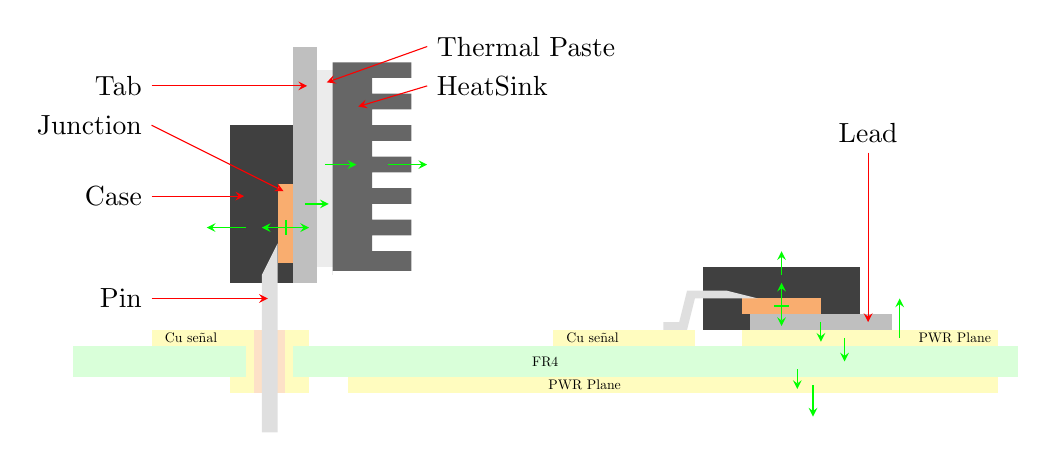
\begin{tikzpicture}[]

	\draw[draw=none,fill=green!15] (-6,-.2) rectangle +(12,.4);
	\draw[draw=none, fill=yellow!25] (-5,0.2) rectangle +(2,.2);
	\draw[draw=none, fill=yellow!25] (-2.5,-0.4) rectangle +(8.25,0.2);

	\node[scale=0.5] at(0,0){FR4};
	\node[scale=0.5] at (-4.5,.3){Cu señal};
	\node[scale=0.5] at (0.5,-.3){PWR Plane};
	\begin{scope}[shift={(-1,0)}]
		% TO-220
		\draw[draw=none,fill=black!75] (-3,1) rectangle +(.8,2);
		\draw[draw=none,fill=gray!50] (-2.2,1) rectangle + (0.3,3);
		\draw[draw=none, fill=Apricot] (-2.4,1.25) rectangle +(.2,1);
		\draw[draw=none,fill=gray!15] (-1.9,1.2) rectangle +(0.2,2.5);
		\draw[draw=none,fill=black!60](-1.7,1.1) -- ++(0,2.7)
		-- ++(1,0) -- ++(0,-.2) -- ++(-0.5,0) -- ++(0,-0.2)
		-- ++(0.5,0) -- ++(0,-.2) -- ++(-0.5,0) -- ++(0,-0.2)
		-- ++(0.5,0) -- ++(0,-.2) -- ++(-0.5,0) -- ++(0,-0.2)
		-- ++(0.5,0) -- ++(0,-.2) -- ++(-0.5,0) -- ++(0,-0.2)
		-- ++(0.5,0) -- ++(0,-.2) -- ++(-0.5,0) -- ++(0,-0.2)
		-- ++(0.5,0) -- ++(0,-.2) -- ++(-0.5,0) -- ++(0,-0.2)
		-- ++(0.5,0) -- ++(0,-.25) -- ++(-1,0);
		\draw[draw=none,fill=yellow!25] (-2.3,-0.4) rectangle +(0.1,0.6);
		\draw[draw=none,fill=yellow!25] (-2.8,-0.4) rectangle +(0.1,0.6);
		\draw[draw=none,fill=yellow!25] (-3,-0.4) rectangle +(1,0.2);
		\draw[draw=none,fill=Apricot!35] (-2.7,-.4) rectangle +(0.4,0.8);
		\draw[draw=none, fill=gray!25] (-2.4,1.5) -- ++(-.2,-.4) -- ++(0,-2) -- ++(0.2,0) -- ++(0,2.4);
		
		\node(th-J) at (-2.2,2.1){};
		\node(th-Tab) at (-1.9,3.5){};
		\node(th-Case) at (-2.7,2.1){};
		\node(th-Pin) at (-2.4,0.8){};

		\node(th-Tp) at (-1.9,3.5){};
		\node(th-HS) at (-1.5,3.2){};
		
		\draw[green,|-stealth] (-2.3,1.7) -- ++(0.3,0);
		\draw[green,-stealth] (-2.05,2) -- ++(0.3,0);
		\draw[green,-stealth] (-1.8,2.5) -- ++(0.4,0);
		\draw[green,-stealth] (-1.,2.5) -- ++(.5,0);

		\draw[green,-stealth] (-2.3,1.7) -- ++(-0.3,0);
		\draw[green,-stealth] (-2.8,1.7) -- ++(-0.5,0);
		

	\end{scope}
	\begin{scope}[shift={(3,.4)}]
		\draw[draw=none,fill=black!75] (-1,0) rectangle +(2,.8);
		\draw[draw=none,fill=gray!50] (-.4,0) rectangle +(1.8,.2);

		\draw[draw=none, fill=Apricot] (-0.5,.2) rectangle +(1,.2);
		\draw[draw=none, fill=gray!25] (-0.3,.4) -- ++(-.4,0.1)
		-- ++(-.5,0) -- ++(-.1,-.4) -- ++(-.2,0) -- ++(0,-.1)
		-- ++(.3,0) -- ++(.1,.4) -- ++(0.8,0);
		\draw [draw=none, fill=yellow!25] (-2.9,0) rectangle +(1.8,-0.2);
		\draw [draw=none, fill=yellow!25] (-0.5,0) rectangle +(3.25,-0.2);
		\node[scale=0.5] at (-2.4,-.1){Cu señal};
		\node[scale=0.5] at (2.2,-.1){PWR Plane};

		\draw[green, |-stealth] (-0,0.3) -- ++(0,0.3);
		\draw[green,-stealth] (0,0.7) -- ++(0,0.3);
		\draw[green, |-stealth] (-0,0.3) -- ++(0,0-.25);
		\draw[green,-stealth] (0.5,0.1) -- ++(0,-0.25);
		\draw[green,-stealth] (0.8,-0.1) -- ++(0,-0.3);
		\draw[green,-stealth] (1.5,-0.1) -- ++(0,0.5);
		\draw[green,-stealth] (0.2,-0.5) -- ++(0,-0.25);
		\draw[green,-stealth] (0.4,-0.7) -- ++(0,-0.4);

		\node(txt-lead) at(1.1,2.5) {Lead};
		\draw[red,-stealth] (txt-lead.south) -- (1.1,0.1);
	\end{scope}

	\node[left](txt-th-J) at (-5,3)  {Junction};
	\node[left](txt-th-Tab) at (-5,3.5)  {Tab};
	\node[left](txt-th-Case) at (-5,2.1)  {Case};
	\node[left](txt-th-Pin) at (-5,0.8)  {Pin};

	\draw[red,-stealth] (txt-th-J.east)-- (th-J);
	\draw[red,-stealth] (txt-th-Tab.east)-- (th-Tab);
	\draw[red,-stealth] (txt-th-Case.east)-- (th-Case);
	\draw[red,-stealth] (txt-th-Pin.east)-- (th-Pin);


	\node[right](txt-th-Tp) at (-1.5,4)  {Thermal Paste};
	\node[right](txt-th-HS) at (-1.5,3.5)  {HeatSink};
	\draw[red,-stealth] (txt-th-Tp.west)-- (th-Tp);
	\draw[red,-stealth] (txt-th-HS.west)-- (th-HS);
\end{tikzpicture}
    \caption{Origen del modelo a partir de componentes}
    \label{fig:ThermalModelOrigin}
\end{figure}

Este modelo se ha basado en la explicacion dada por la AN-2020\cite{TiAN2020} de Texas Instruments.


\subsubsection{Modelo completo}
A partir del modelo anterior podemos añadir un dispipador encima del chip y otro por debajo de la PCB con lo que el modelo quedaria:

\begin{figure}[H]
    \centering
    % !TeX encoding = UTF-8
% !TeX spellcheck = es_ES
% !TeX root = ../Thermal.tex
%!TEX root=../Thermal.tex

\begin{tikzpicture}[american]

\begin{scope}[shift={(0,0)}]
			%\draw (-6,-6.5) rectangle +(12,13);
			
			\draw (-5.25,5.5)
				to[isource, l=$W$ ] ++(2.5,0)
					coordinate(TJ) 
				node [red, above] {$T_{j}$}
				to [R,l=$R_{thJC}$] ++(0,-2.5) 
					coordinate(TC)
				node[red,above left]{$T_{case}$}
				to [R,l=$R_{thCA}$] ++ (0,-6)
					coordinate(TA)
				node[red,above left]{$T_{amb}$}
				to[vsource,v=$T_{amb}$] ++(0,-2.5)
				node[ground]{};
			
			\draw[gray] (TC) to[short,*-] ++(-2.5,0)
				to[R,l=$R_{thCHs}$,-*,color=gray] ++(0,-3)
				coordinate(THst)
				node[red, left]{$T_{Hst}$}
				to[R,l=$R_{thHst}$, color=gray] ++(0,-3)
				to[short,-*](TA);

			\draw (TJ) to[short,*-] ++(2.5,0)
				to[R,l=$R_{thJL}$] ++(0,-2.5)
					coordinate(TL)
					node[red,right]{$T_l$}
				 to [R,l=$R_{thSn}$] ++ (0,-2)
					coordinate(Ttop)
					node[red,left]{$T_{top}$}
				to[R,l=$R_{thPt}$,-*]++(0,-4)
				to[short,-*](TA);
			
			\draw[dotted] (TL)to[R,l=$R_{thLC}$,*-] (TC);
			\draw (Ttop) to [R,l^=$R_{thPtPb}$,*-] ++(3,0)
				coordinate(TPb)
				node[red,above ]{$T_{bott}$}
				to[R,l=$R_{thPb}$,-*] ++(0,-4)
				coordinate(TAr)
				to[short,-*] (TA)
			;

			\draw[gray] (TPb) to[short,*-] ++(2.5,0)
				to[R,l=$R_{thPbHsb}$,-*, color=gray] ++(0,-2)
				coordinate(THsb)
				node[red,right]{$T_{Hsb}$}
				to[R,l=$R_{thHsb}$, color=gray] ++(0,-2)
				to[short] (TAr);

			%\draw (TC) to[short,*-] ++(2,0)
			%	to[R,l=$R_{thS}$] ++(0,-2.)
			%	to[R,l=$R_{thHS}$] ++(0,-2.)
			%	to[short,-*](TA);
			
     \end{scope}

\end{tikzpicture}



    \caption{Modelo más complicado a usar}
    \label{fig:ThermalModelFull}
\end{figure}

Este modelo es el mas complicado que debemos tener en cuenta para un proyecto hobby que entre dentro
del paraguas Dcc Diy Tools. Si necesitamos complicarlo más habria que considerar usar software
profesional\sidenote{Que lo hay}.

En general los valores de las resistencias son:

\begin{subequations}
    \label{eq:ResRthVal}
    \begin{align}
		\label{eq:RJunctionToCase}
			R_{thJC}	\simeq R_{thJL} & \approx 15 &&   10<R_{thJC/L} <20 \\
		\label{eq:RThermalPaste}
			R_{thCHs} \simeq R_{thPbHsB} &\approx 0.8 && 0.5\leq R_{thTP} \leq 1\\
		\label{eq:RPcb}
			R_{thPt}\simeq R_{thB}&=\frac{\alpha}{Area} && R_{th}(a)=\frac{100}{a_{Inch^2}} = \frac{100}{a_{cm^2}/6}=\frac{600}{a_{cm^2}}\\
   	\label{eq:ResTopBottom}
			R_{thPtPb}&=f(mat,vias) && R_{thPtPb}(fr4,0) \approx 10 \\
		\label{eq:ResSnValue}
			R_{Sn}& \approx 0.1 && 0< R_{sn} <1
	\end{align}
\end{subequations}
\begin{center}
Valores tipicos
\end{center}

La equacion \ref{eq:RJunctionToCase} se refiere a que la resistencia del Silicio a un pin es similar
a la resistencia del mismo carcasa, siendo 15 un valor tipico que nos encontraremos. 
Y en todo caso estara en el rango de 10 a 20.

Las restencias de las pastas termicas \ref{eq:RThermalPaste} seran todas similares,
seguramente 0,8. 

Ademas la resistencia de una zona de cobre, es inversamente proporcinal a su area, con un valor de 
\SI{100}{\celsius\per\watt} cada incha cuadrada o 6 centimetros cuadrados. Ademas la resistencia
termica entre la capa supererior e inferior depende del material de la placa y de las vias utilizadas,
Si no hay vias, una placa de fr4 de \SI{1.6}{\mm} tiene un valor de \SI{10}{\celsius\per\watt}.

Por ultimo el estaño que une el pin al pad de cobre, tiene una resitencia minima, casi cercana
a 0.

Teniendo en cuenta los valores y su proporcion con otras Resistencias se puede simplificar este
circuito, de forma general y especifica segun se usen disipadores o no.

\begin{subequations}
    \label{eq:ResRth}
    \begin{align}
		\label{eq:RCaseToLead}
			R_{thLC}\gg R_{thJC} & & & R_{thLC}\approx \infty \\
		\label{eq:RThermalHst}
			R_{thCHs}\ll R_{thHst}&  && R_{thCHs}\approx 0\\
		\label{eq:RThermalHsb}
			R_{thPbHsb}\ll R_{thHsb}&  && R_{thPbHsb}\approx 0 \\
		\label{eq:RSolder}
			R_{thSn}\ll R_{thJL} & & & R_{thSn} \approx 0
   \end{align}
\begin{center}
Simplificaciones globales
\end{center}
\end{subequations}

Por otra parte \ref{eq:RCaseToLead}, $R_{thLC}$ respecto a las otras resistencias es lo suficientemente grande
como para considerar que es un circuito abierto o de valor infinito.

El valor de la pasta termica sera pequeño comparado con la del disipador al que
acompañan que pueden obviarse. Ya sea encima del componente \ref{eq:RThermalHst} o por debajo
de la pcb \ref{eq:RThermalHsb}. 

Algo paracido pasa con la Resitencia del estaño usado para unir el chip a la PCB.
Es tan pequeño respecto a otras resistencias que se puede obviar \ref{eq:RSolder}

Finalmente se suelen seguir una serie de reglas de diseño que pueden simplificar aun más el diseño.
Para empezar cuando se decide disipar el calor. Se escoge un solo camino de los siguientes:

\begin{itemize}
	\item \textbf{Disipador Superior}: En este caso se busca un Disipador cuya $R_{th}$ sea tan pequeña
que deprede todas las demas. La PCB no se diseña para disipar calor.

\begin{subequations}
    \begin{align}
		\label{eq:RCaseVsLead}
			R_{thRamaCase}&\ll R_{thRamaLead} & & R_{thRamaLead}\approx \infty\\
		\label{eq:RthHsOverridesCA} R_{thCHs} + R_{thHs} &\ll R_{thCA} & & R_{thCA} \approx \infty \\
		\label{eq:RthDispidadorSuperior}
			R_{thJA}=R_{thJC}&+R_{th_CHs}+R_{thHs} && R_{thJA}=R_{thJC}+R_{thHs}
   \end{align}
\begin{center}
Simplificaciones Disipador Superior
\end{center}
\end{subequations}
En este caso, al no haberse diseñado la pcb como disipador, la resitencia por la rama de la misma sera muy alta (en comparacion con la rama del dispador), tanto que se puede considerar que no
exista \ref{eq:RCaseVsLead}. Lo mismo pasa con la disipacion de la carcasa. Una buena eleccion del
dispador hace que podamos ignorar la disipacion por la carcasa \ref{eq:RthHsOverridesCA}  y nos queda una ecuacion de tres
resistencias, \ref{eq:RthDispidadorSuperior} y a tenor de sus valores \ref{eq:RThermalHst} podemos resumir en la ecuacion con solo dos resitencias

\item \textbf{Disipador Inferior}: Otra forma de disipar el calor en componentes SMD es usar un
dispador por la cara opuesta donde esta montando el chip. Esta solucion requiere ocupar con cobre
descubierto en la capa inferior del mismo tamaño que el disipador. Y en la capa supererior que los 
pads "termales" \sidenote{Mirar el datasheet} sean lo suficentemente grandes como para poner las
vias adecuadas, asi las capas superior e inferior tiene una buena conductividad termica.

\begin{subequations}
    \begin{align}
		\label{eq:RCaseVsLead2}
			R_{thRamaLead}&\ll R_{thRamaCase} & & R_{thRamaCase}\approx \infty\\
		\label{eq:RthPtPbGood}
			R_{thPtPb}&=R_{th}(fr4,OptimunVias) && R_{thPtPb}\approx 0 \\
		\label{eq:BottomHSOverrides}
			R_{thHsb} &\ll R_{thPt} || R_{thPb} && R_{thPt} \sim R_{thPb} \approx\infty \\ \label{eq:RthDispidadorSuperior}
			R_{thJA}=R_{thJL}&+R_{th_PbHsb}+R_{thHsb} && R_{thJA}=R_{thJL}+R_{thHsb}
   \end{align}
\begin{center}
Simplificaciones Disipador Superior
\end{center}
\end{subequations}



A pesar de que la superficie de cobre mejorara la disipacion de calor, es el disipador quien hara el trabajo, con un valor mucho menor .
\end{itemize}
 




\subsection{Modelo Simplificado}
% !TeX encoding = UTF-8
% !TeX spellcheck = es_ES
% !TeX root = ../Thermal.tex
%!TEX root=../Thermal.tex
El modelo más simplificado es una resistencia, que podremos usarlo cuando este dato nos sea dado
por el fabricante en el DataSheet.
El más realista son dos resistencias en serie, una representado la resistencia desde el silicio al
disipador (ya sea, la carcasa, la pcb o un trozo de metal) y otra de este ultimo al aire.



\begin{figure}[H]
    \centering
    % !TeX encoding = UTF-8
% !TeX spellcheck = es_ES
% !TeX root = ../Thermal.tex
%!TEX root=../Thermal.tex

\begin{tikzpicture}[american]
    %\draw (0,0) circle[radius=1pt];
    \begin{scope}[shift={(-5,0)}]
        %\draw (0,0) circle[radius=1pt];
        %\draw (-2.5,-3.5) rectangle +(5,7);
        
        \draw (-2,2.5) to[isource, l=$W$ ] (0.5,2.5)
            node[right,red]{$T_j$} 
            to[R, l2=$R_{thJA}$ and $\si{\degree\kelvin\per\watt}$] (0.5,-0)
            node[right,red]{$T_{amb}$} 
            to[vsource=$T_a$] (0.5,-2.5)
            node[right,red]{$\SI{0}{\celsius}$} 
            node[ground](gnd){};
        \node at(0,-3.5) {a) Simplificado};
    \end{scope}


    \begin{scope}[shift={(-0,0)}]
        %\draw (0,0) circle[radius=1pt];
        %\draw (-2.5,-4.75) rectangle +(5,9.5);
        
        \draw (-2,3.75) to[isource, l=$W$ ] (0.5,3.75)
            node[right,red]{$T_j$} 
            to[R, l2=$R_{thJC}$ and $\si{\degree\kelvin\per\watt}$] (0.5,1.25)
            node[right,red]{$T_{case}$} 
            to[R, l2=$R_{thCA}$ and $\si{\degree\kelvin\per\watt}$] (0.5,-1.25)
            node[right,red]{$T_{amb}$} 
            to[vsource=$T_a$] (0.5,-3.75)
            node[right,red]{$\SI{0}{\celsius}$} 
            node[ground](gnd){};
        \node at(0,-4.75) {b) Normal};
    \end{scope}

    \begin{scope}[shift={(5,0)}]
        %\draw (0,0) circle[radius=1pt];
        %\draw (-2.5,-3.5) rectangle +(5,7);
        
        \draw (-2,3.75) to[isource, l=$W$ ] (0.5,3.75)
            node[right,red]{$T_j \leq \SI{125}{\celsius}$} 
            to[R, l2=$R_{thJC}$ and $\si{\degree\kelvin\per\watt}$] (0.5,1.25)
            node[right,red]{$T_{case} \leq \SI{100}{\celsius}$} 
            to[R, l2=$R_{thHS}$ and $\si{\degree\kelvin\per\watt}$] (0.5,-1.25)
        
            node[right,red]{$T_{amb}\approx \SI{25}{\celsius}$} 
            to[vsource=$T_a$] (0.5,-3.75)
            node[right,red]{$\SI{0}{\celsius}$} 
            node[ground](gnd){};
        \node at(0,-4.75) {c) Usable};
    \end{scope}

\end{tikzpicture}

    \caption{Circuito Equivalente}
    \label{fig:ThermalEquivalent}
\end{figure}

En la practica es mejor modelar como dos resistencias, una $R_{thJC}$ :
Junction\sidenote{El silicio} a la case\sidenote{Carcasa} y $R_{thCA}$ de la
carcasa al ambiente, tal y como se representa en el caso (b) \ref{fig:ThermalEquivalent}.
De esta forma podremos variar $R_{thCA}$ con un dispador más grande.

En este modelo es importante mantener la temperatura del silicio $T_j$ por debajo de
$\SI{125}{\celsius}$ lo que se suele corresponde con $T_c=\SI{100}{\celsius}$ en la carcasa.
Como hemos visto, en la realidad, el modelo es más complejo, con resistencias en paralelo segun el dispador
que se ponga, pero se simplifica por la diferencia valores y se puede ignorar $R_{thCA}$
por $R_{thHS}$ del disipador\sidenote{HeatSink}.


\subsection{Calculos en la practica}
% !TeX encoding = UTF-8
% !TeX spellcheck = es_ES
% !TeX root = ../Thermal.tex
%!TEX root=../Thermal.tex
Generalmente querremos saber si nuestro diseño es viable, pero podemos concretar
en que queremos responder una de estas preguntas:
\begin{itemize}
    \item ¿Cuanta es la potencia maxima que podemos usar en este componente?
    \item ¿Que temperatura alcanzara el componente con la potencia que va a pasar?
          o cada parte (carcasa, pcb, \dots)
    \item ¿Cual es el disipador minimo que tenemos que poner? o que es lo mismo
          ¿Que resistencia maxima debe tener el disipador?
    \item ¿Que area minima debemos usar en la PCB para disipar X potencia?
\end{itemize}

La mejor forma de conseguir esto es diseñar una PCB pequeña, de tamaño similiar
al standart JESD51 de JEDEC, pero modificada para que se parezca a nuestra PCB
final y probar con una fuente de laboratorio y una camara de infrarojos. La segunda
mejor forma es sobre nuestras PCB.

Aunque hoy por hoy es barato obtener una PCB, es mucho mas rapido hacer unos pocos
calculos y luego comprobarlos sobre la PCB. Los componentes siguen teniendo un precio

Para cualquier pregunta, deberemos trabjar con el modelo de una o dos resistencias.
Para ello trabajaremos solo con un camino de disipacion y obviaremos el otro.

En el caso de los componentes through hole solo tenemos dos opciones, con o sin
disipador. Si no tenemos dispador solo tendremos el camino por la carcasa al
aire, pero si ponemos un disipador tenemos  dos caminos. En este caso podemos
eliminar el camino que va por la carcasa.

En cambio, para los componentes SMD, siempre tendremos la disipacion por PCB,
aunque no añamos diseñado la PCB como disipador. Si no hemos diseñado la PCB
a conciencia\sidenote{Podria ser que sin querer sea un buen disipador} solo
tenedremos en cuenta la disipacion por la carcasa. Y si nuestra intencion es
usar la PCB como disipador, es mejor descartar la carcasa y diseñar la PCB
como unica opcion de disipador.

Al omitir un camino lo que conseguimos es un error al alza en la temperatura
por lo que si nuestro diseño es seguro\sidenote{$T_j< \SI{125}{\celsius}$}
segun los calculos lo sera en la realidad.

Como ejemplo vamos usar un chip 78XX de onsemi, MC7800 cuyo datasheet nos dice
lo siguiente:
\begin{table}[H]
    \centering
    \renewcommand\theadfont{\bfseries}
    \setlength{\tabcolsep}{10pt}
    \renewcommand{\arraystretch}{1.5}
    \begin{tabular}{|l|c|c|c|c|}
        \hline
                                  &                          &            & \multicolumn{2}{|c|}{Empaquetado}                      \\ \hline
        desc                      & PadSize                  & Symbol     & TO-220                            & \makecell{TO-252-3 \\ DPAK } \\ \hline
        Th R, Junction-to-Case    &                          & $R_{thJC}$ & 5                                 & 5                  \\ \hline
        Th R, Junction-to-Ambient &                          & $R_{thJA}$ & 65                                & 96                 \\ \hline
        Th R, Junction-to-Ambient & $5*\SI{5}{\square\mm}$   & $R_{thJA}$ & -                                 & 67                 \\ \hline
        Th R, Junction-to-Ambient & $10*\SI{10}{\square\mm}$ & $R_{thJA}$ & -                                 & 56                 \\ \hline
        Th R, Junction-to-Ambient & $20*\SI{20}{\square\mm}$ & $R_{thJA}$ & -                                 & 49                 \\ \hline
        Max Junction Temperature  &                          & $T_j$      & 150                               & 150                \\
        \hline
    \end{tabular}
    \caption{Datos suministrados por el DataSheet}
    \label{tab:MC7800_ds_thermal_data}
\end{table}

Como podemos ver no nos dice $R_{thCA}$ ni $R_{thPCB}$ y tenemos diferentes $R_{thJA}$
segun el tamaño del pad. Con esta informacion podemos averiguar los datos que nos faltan
usando las siguentes formulas.


\begin{subequations}
    \label{eq:basicRth}
    \begin{align}
        \label{eq:RthSinDisipador} R_{thJA}          & =R_{thJC}+R_{thCA}                     &  & \text{Sin disipador }     \\
        \label{eq:RthConDisipador} R_{thJA}(a_{pcb}) & =R_{thJC}+R_{thCA}||R_{thPCB}(a_{pcb}) &  & \text{Con disipador(PCB)}
    \end{align}
\end{subequations}

De las cuales podemos deducir las siguientes ecuaciones:

\begin{subequations}
    \label{eq:ResRth}
    \begin{align}
        \label{eq:RthJA} R_{thCA}            & =R_{thJA}-R_{thJC}                                                    \\
        \label{eq:RthPcb} R_{thPcb}(a_{pcb}) & =\frac{1}{\frac{1}{R_{thJA}(a_{pcb}) - R_{thJC}} -\frac{1}{R_{thCA}}}
    \end{align}
\end{subequations}

Siguiendo los siguientes pasos:

\begin{align*}
    R_{thCA}                               & =R_{thJA}-R_{thJC}                                                    &  & \text{Despejando de \ref{eq:RthSinDisipador}}      \\
    \\
    R_{thJA}(a_{pcb})                      & =R_{thJC}+\frac{1}{\frac{1}{R_{thCA}}+\frac{1}{R_{thPcb}(a_{pcb})}}   &  & \text{Applicando  || en  \ref{eq:RthConDisipador}} \\
    R_{thJA}(a_{pcb}) - R_{thJC}           & =\frac{1}{\frac{1}{R_{thCA}}+\frac{1}{R_{thPcb}(a_{pcb})}}            &  & \text{Despejando}                                  \\
    \frac{1}{R_{thJA}(a_{pcb}) - R_{thJC}} & = \frac{1}{R_{thCA}}+\frac{1}{R_{thPcb}(a_{pcb})}                     &  & \text{Aplicando $1/x$}                             \\
    \frac{1}{R_{thPcb}(a_{pcb})}           & =\frac{1}{R_{thJA}(a_{pcb}) - R_{thJC}} -\frac{1}{R_{thCA}}           &  & \text{Despejando}                                  \\
    R_{thPcb}(a_{pcb})                     & =\frac{1}{\frac{1}{R_{thJA}(a_{pcb}) - R_{thJC}} -\frac{1}{R_{thCA}}} &  & \text{Aplicando $1/x$}
\end{align*}

Con estas ecuaciones obtenemos los datos que nos faltan:

\begin{table}[H]
    \centering
    \renewcommand\theadfont{\bfseries}
    \setlength{\tabcolsep}{10pt}
    \renewcommand{\arraystretch}{1.5}
    \begin{tabular}{|l|c|c|c|c|}
        \hline
                              &                      &            & \multicolumn{2}{|c|}{Empaquetado}                      \\ \hline
        desc                  & PadSize              & Symbol     & TO-220                            & \makecell{TO-252-3 \\ DPAK } \\ \hline
        Th R, Case-to-Ambient &                      & $R_{thCA}$ & 60                                & 91                 \\ \hline
        Th R, Case-to-Ambient & 5x5\si{\square\mm}   & $R_{thCA}$ & -                                 & 195                \\ \hline
        Th R, Case-to-Ambient & 10x10\si{\square\mm} & $R_{thCA}$ & -                                 & 122                \\ \hline
        Th R, Case-to-Ambient & 20x20\si{\square\mm} & $R_{thCA}$ & -                                 & 86                 \\ \hline
    \end{tabular}

    \caption{Datos suministrados por el DataSheet}
    \label{tab:MC7800_calc_thermal_data}
\end{table}

\subsubsection{Maxima Potencia}
% !TeX encoding = UTF-8
% !TeX spellcheck = es_ES
% !TeX root = ../../Thermal.tex
%!TEX root=../../Thermal.tex

Para calcular la potencia maxima que se puede disipar para una configuracion dada conviene
calcular la $R_{thJA}$ equivalente, ya sea realizando toda la simplificacion o empiricamente.
Una vez calculada dicha Resistencia es cuestion de despejar:

\begin{align*}
	T_j=T_{amb}+W_{max} \cdot R_{thJA} & & \text{Original} \\
	125&=25+W_{max} \cdot R_{thJA} & & \text{Sustituimos limite} \\
\frac{125-25}{R_{thJA}}&=W_{max} & & \text{Despejamos}
\end{align*}
Con lo que llegamos a la ecuacion \ref{eq:ResMaxWatt}:
\begin{equation}
\label{eq:ResMaxWatt}
W_{max}=\frac{100}{R_{thJA}}
\end{equation}


\subsubsection{Temperatura de cada elemento}
% !TeX encoding = UTF-8
% !TeX spellcheck = es_ES
% !TeX root = ../../Thermal.tex
%!TEX root=../../Thermal.tex
Algunas veces conviene pararnos a pensar si nuestro diseño actual es seguro
para el chip, debemos ver a que temperatura llega cada parte del diseño. 

Asi que para calcular la temperatura de diversos puntos del chip, como la carcasa, la
parte superior de la pcb,\dots, se debe escoger el modelo que más se adecue a
los puntos a calcular y resolver.

Partiremos siempre de la premisa de que la placa se ha diseñado para disipar
calor ya sea por tener un dispador o por suficiente superficie en la placa
que sea disipadora. Y a partir de ahi simplifcar el circuito termico. Todo
aquello que no se haya pensado como dispador, debe ser excluido del modelo.

La primera simplificacion.




